\chapter{開発手法}
\label{chap:coding}

本章ではDreamMemoryの概要、利用方法、システム概要について述べる。

\section{概要}
 現在、拡張現実を体験すべくOculous Riftなどのヘットマウントディスプレーをはじめとして様々なツールが開発されている。そこで本研究では睡眠中の夢を自由にコントロールする方法があれば誰もがより簡単に拡張現実を体験をすることができるのではないかと考えた。そこで眠っっている時にその人が過去に体験したことと関連した音を流すことで、その音に基づいて夢を見ることを促進するスマートフォンアプリDreamMemoryを試作した。\\
 DreamMemoryのターゲットユーザーは日々のストレスから解放されたい人、懐かしい思い出をもう一度体験したい人、物理的に会えない人と会いたい人などが含まれる。\\
 DreamMemoryには3つ主要な機能がある。一つ目は寝る前に印象に残っている記憶に関する写真と映像を表示する機能。二つ目は睡眠中にREM睡眠を検出し、記憶を連想させる音を流す機能。例えば特別な誰かを連想する音、旅行中によく聞いていた曲、最寄り駅の音楽、好きな映画のサウンドトラックなどだ。三つ目は起床後に夢について記録する夢日記機能である。ユーザーには睡眠前にスマートフォンを画像\ref{DreamMemoryImage}のように枕の横に置いてもらう。\\
 DreamMemoryは開発途中でまだAppストアには掲示していないが、githubからソースコードを入手することができる。iOSスマートフォンを持っていて、Apple Developerの登録をしている人であればインストールできるようになっている。

\begin{figure}[htbp]
\begin{center}
\includegraphics[width=14cm]{eps/dreamDate02.eps}
\caption{DreamMemory:枕の横に配置して、ユーザの体動を観測する}
\label{DreamMemoryImage}
\end{center}
\end{figure}

\section{利用方法}
 ユーザーには予め記憶を思い起こさせる音を登録してもらう。音選びは適している音声と適さない音声があるため注意する必要がある。使用してはいけない音は人の声だ。特に喋りかけてくるような内容の音声は、ユーザーを起こしてしまう可能性が高いということが実験結果から分かった。詳しくは第6章で述べる。逆に適している音は繰り返しある環境下で聞いていた音である。
 アプリの起動後、\ref{le01}のような画面が表示される。そこには「自動ロック機能をOFFにする」「音量は1〜3に設定する」やiPhoneの置く位置などの指示が書かれている。次に\ref{le02}の画面に遷移し、ユーザーの思い出に関連性のある画像を表示する。ここでは寝る前に記憶の情景を思い出す機会を与えている。そして\ref{le03}の画面では思い出の音楽が流れる。音楽を聴きながら、旅先での空間、香り、音の細部までを思い出して、気持ちを落ちつかせて瞑想状態に入ってもらう。次に\ref{le04}の画面に移動する。ユーザーは寝る前にアプリを起動してスタートボタンを押し、起動させたままスクリーンを伏せて枕の横に置く。20〜30分間後にDreamMemoryの加速度が起動をし一晩中ユーザーの体動のトレッキングが行われ、REM睡眠を検知すると音楽がなる。起床後\ref{le05}の画面で、ユーザーは起床すると夢の内容を忘れないように日記に投稿する。

\begin{figure}[htbp]
 \begin{minipage}{0.45\hsize}
  \begin{center}
   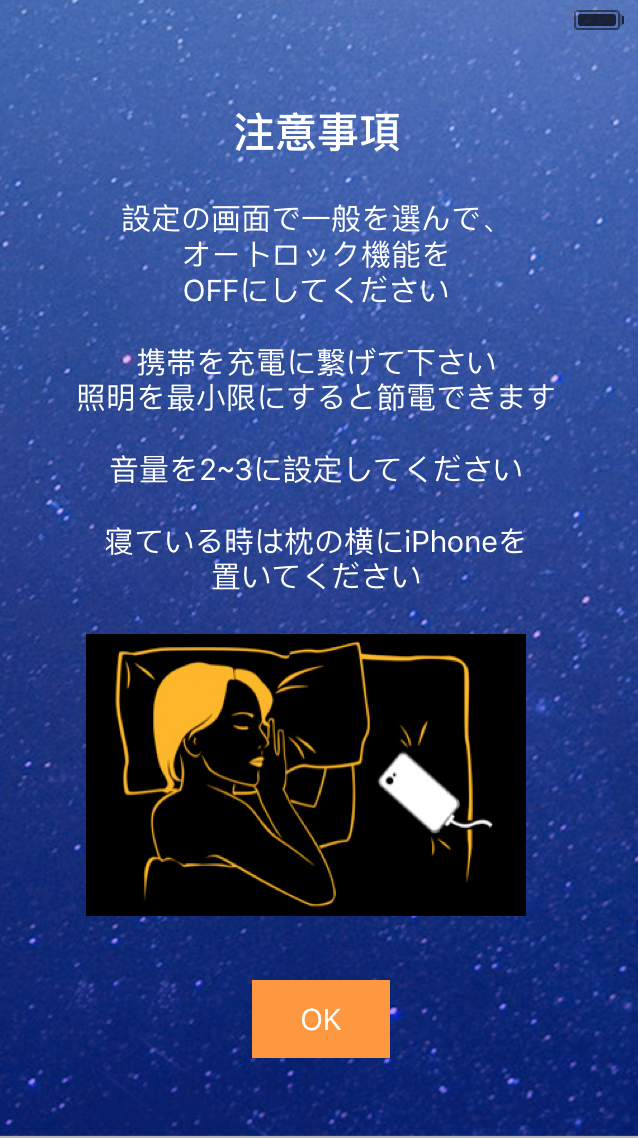
\includegraphics[height=90mm]{eps/AppIntro.eps}
  \end{center}
  \caption{起動画面}
  \label{le01}
 \end{minipage}
 \begin{minipage}{0.45\hsize}
  \begin{center}
   \includegraphics[height=90mm]{eps/AppMemoryImages.eps}
  \end{center}
  \caption{思い出の画像を表示}
  \label{le02}
 \end{minipage}
\end{figure}

\begin{figure}[htbp]
 \begin{minipage}{0.45\hsize}
  \begin{center}
   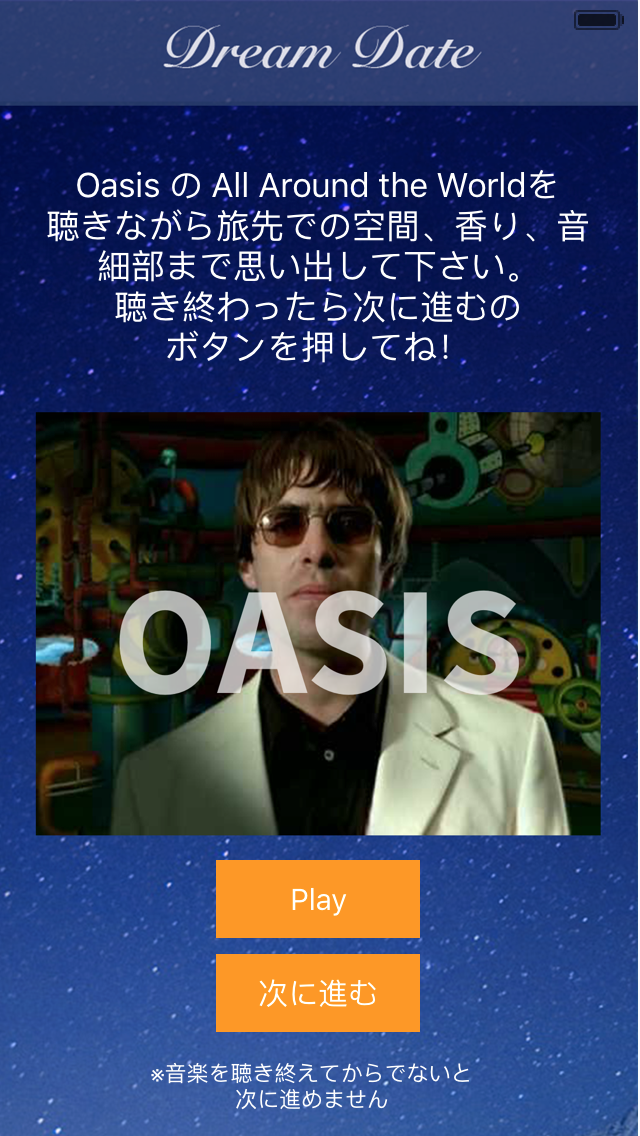
\includegraphics[height=90mm]{eps/AppMusicPlay.eps}
  \end{center}
  \caption{思い出の音楽が流れる}
  \label{le03}
 \end{minipage}
 \begin{minipage}{0.45\hsize}
  \begin{center}
   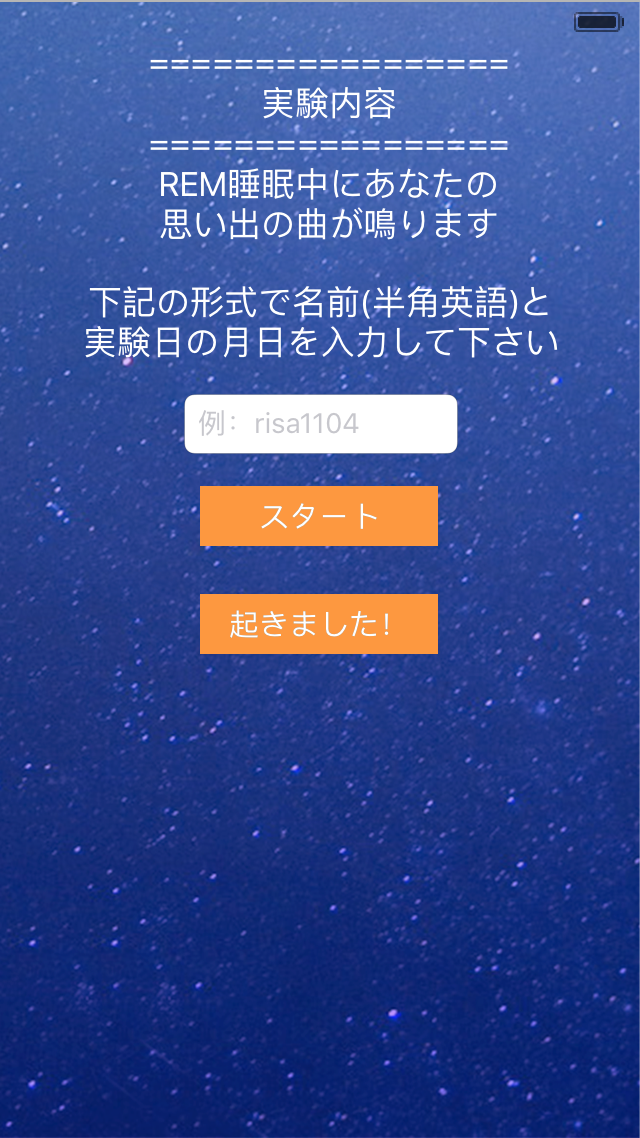
\includegraphics[height=90mm]{eps/AppStart.eps}
  \end{center}
  \caption{眠り開始ボタン}
  \label{le04}
 \end{minipage}
\end{figure}

\begin{figure}[htbp]
 \begin{minipage}{0.45\hsize}
  \begin{center}
   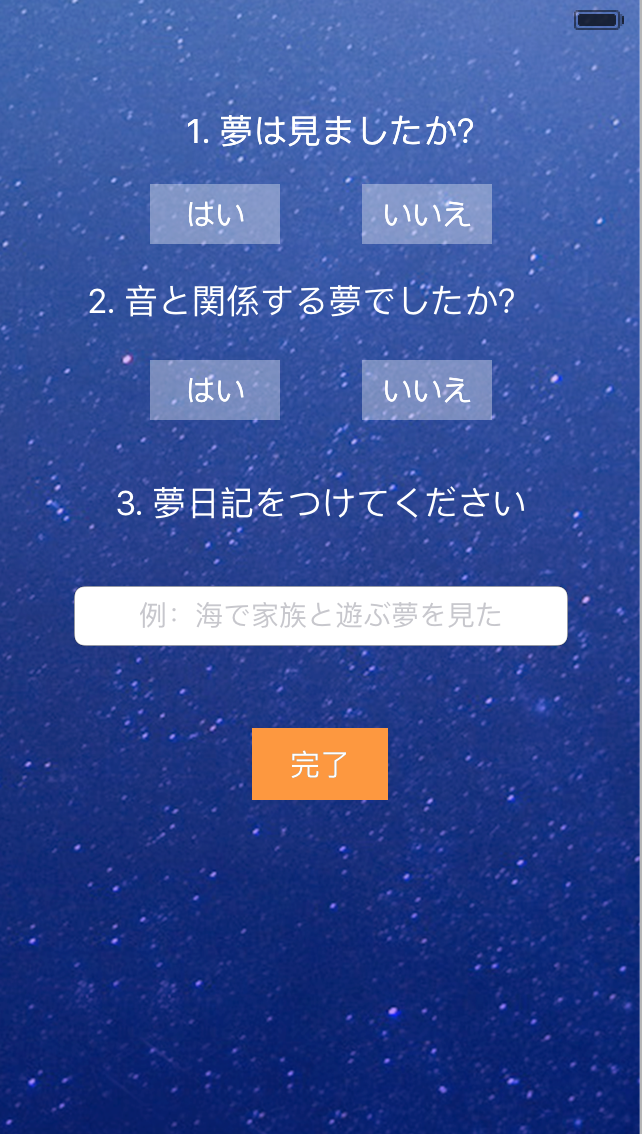
\includegraphics[height=90mm]{eps/AppDiary.eps}
  \end{center}
  \caption{夢日記記入ページ}
  \label{le05}
 \end{minipage}
 \begin{minipage}{0.45\hsize}
 \end{minipage}
\end{figure}

\section{システム概要}
\subsection{センシングの方法とその正確性}
 DreamMemoryでは記憶を思い起こさせる音声をコンテンツをREM睡眠を感知した際に流すことで、ユーザーの夢を操作することを目指す。REM睡眠の感知はスマートフォンに備わっている加速度センサーを使用した。\\

MemoryDreamは寝返りを検知するシステムになっているが、これもユーザごとにキャリブレーションを行って、正確に寝返りを検知できるようにした。以下の図\ref{sensing}はMemoryDreamのセンシング結果を他のアプリケーションと比較したものだが、非常に近いデータの結果が出たことがわかる。

\begin{figure}[htbp]
\begin{center}
\includegraphics[width=10cm]{eps/sensing.eps}
\caption{センシング部分の他のアプリとの比較}
\label{sensing}
\end{center}
\end{figure}